\chapter{Obecnie stosowane generatory liczb losowych}\label{ch:przeglad-rynku}

Współczesne systemy kryptograficzne oraz aplikacje wymagają generowania liczb losowych,
które muszą charakteryzować się wysoką jakością i odpornością na przewidywalność.
Najlepiej spełniają do generatory liczb prawdziwie losowych, czyli te oparte na fizycznych zjawiskach,
jednak powszechnie używane są generatory pseudolosowe (PRNG, z ang. \textit{Pseudorandom Number Generator}).
PRNG są całkowicie deterministyczne i zależą od zadanej im wartości początkowej zwanej ziarnem (ang. \textit{seed}).

TRNG są szczególnie istotne w kontekście aplikacji wymagających silnej ochrony danych,
takich jak systemy kryptograficzne, podpisy cyfrowe, oraz w generowaniu kluczy szyfrujących.

\section{Obecnie stosowane rozwiązania}\label{sec:obecnie-stosowane-rozwiazania}

%todo - opisać to lepiej, może Kuba (Yoshida) o linuxowych?
Obecnie komputery osobiste wykorzystują generatory liczb losowych (RNG, z ang. \textit{Random Number Generator})
wykorzystujące dostępne im źródła entropii dostarczane przez użytkownika, takie jak ruchy myszy lub naciśnięcia przycisków.
W nowoczesnych procesorach stosuje się też liczby generowane przez dedykowane moduły takie jak \textbf{Intel DRNG} za pomocą \textit{Intel RDSEED} i \textit{RDRAND}~\cite{IntelRD}.
System Linux dostarcza również interfejsy \textit{/dev/random} raz \textit{/dev/urandom} zapewniające liczby losowe.

\section{Przegląd komercyjnych rozwiązań TRNG}\label{sec:przeglad-komercyjnych-rozwiazan-trng}

Komercyjne rozwiązania bazują na przeróżnych źródłach entropii,
najczęściej nie na dostarczanych przez użytkownika, aby wykluczyć możliwość ingerencji i ograniczyć przewidywalność.
Najpopularniejszym medialnie RNG jest LavaRand~\cite{cloudflare_lavarand}, który inspirowany był podobnym systemem,
zbudowanym i opatentowanym przez \textbf{Silicon Graphics}~\cite{SiliconGraphics}.
LavaRand jest dzisiaj jedynie dodatkowym zabezpieczeniem firmy,
na wypadek gdyby ich konwencjonalne źródła entropii okazały się niewystarczające.
Wciąż jednak pozostaje inspirującym przykładem do szukania losowości wszędzie wokół nas.

\begin{figure}[h]
    \centering
    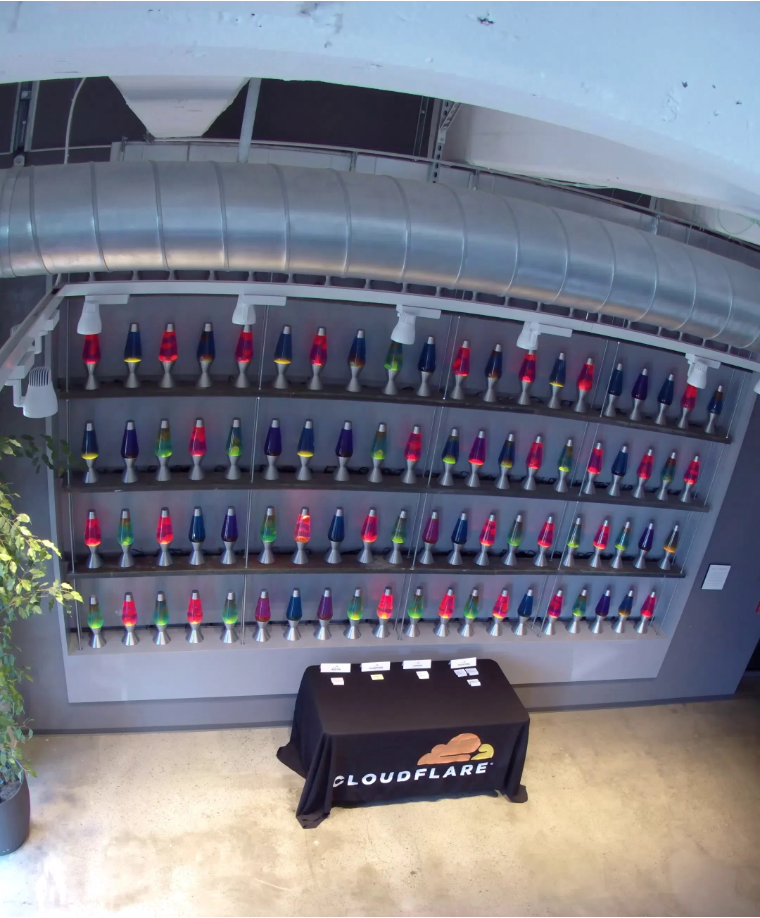
\includegraphics[width=0.4\linewidth]{chapters/02-teoria/figures/lavarandCamera}
    \caption{Widok z kamery w biurze Cloudflare~\cite{cloudflare_lavarand}.}
    \label{fig:lavarand}
\end{figure}

Silicon Graphics oferuje użytkownikom dostęp do generatora liczb losowych w chmurze, który jest wykorzystywany
m.in. do tworzenia kluczy kryptograficznych oraz w innych zastosowaniach wymagających silnych zabezpieczeń.
Dzięki wykorzystaniu globalnej infrastruktury Cloudflare, generowane liczby losowe są
szeroko dostępne i charakteryzują się dużą niezawodnością oraz odpornością na ataki.

W ostatnich latach pojawiły się także inne rozwiązania chmurowe, które umożliwiają generowanie liczb losowych w czasie rzeczywistym bez potrzeby posiadania własnego sprzętu,
za to na przykład za pośrednictwem API takiego jak drand~\cite{drand_documentation} lub podobnego.
% "lub podobnego" źle brzmi
Przykładem takiego rozwiązania jest \textbf{Cloudflare} – firma specjalizująca się w dostarczaniu usług związanych z bezpieczeństwem sieciowym.
Na swoim blogu Cloudflare przedstawia zaawansowane metody generowania liczb losowych, które są wykorzystywane w ich systemach~\cite{cloudflare_league_of_entropy}.
Dodatkowo \textbf{Cloudflare} korzysta z technologii opartych na zjawiskach fizycznych, takich jak rozpad radioaktywnego uranu, 
nieprzewidywalnego fizycznie trójstopniowego wahadła, czy „Entropy Wall”, która pobiera entropię z kamery
ustawionej na ścianę lamp lawowych, pokazanej na rys.~\ref{fig:lavarand}.
Te prawdziwie losowe wartości zostają potem użyte jako ziarno dla generatorów pseudolosowych.
Tego typu rozwiązania pozwalają na szybkie i bezpieczne generowanie liczb losowych w skali globalnej, zapewniając jednocześnie wysoki poziom ochrony przed atakami.

\subsection{Rozwiązania sprzętowe}\label{subsec:rozwiazania-sprzetowe}
Wiodącymi producentami komercyjnych rozwiązań sprzętowych są firmy takie jak
\textbf{ID Quantique}~\cite{IDQ}, \textbf{Microchip Technology}~\cite{MicrochipTechnology} i \textbf{Semtech}~\cite{Semtech},
które oferują zaawansowane urządzenia bazujące na TRNG.
Produkty te zapewniają wysoki poziom bezpieczeństwa i są stosowane w wymagających tego aplikacjach,
takich jak bankowość elektroniczna czy systemy wojskowe.

\begin{itemize}
    \item \textbf{ID Quantique} jest jednym z liderów w dziedzinie generatorów liczb losowych opartych na technologii fotoniki i mechanizmach kwantowych.
     Firma oferuje urządzenia, które wykorzystują detekcję fotonów w celu generowania liczb losowych.
     Dzięki temu rozwiązania ID Quantique charakteryzują się bardzo wysoką jakością losowości,
     a jednocześnie są odporne na ataki związane z analizą i przewidywaniem generowanych liczb.

    \item \textbf{Microchip Technology} w swojej ofercie posiada różne moduły TRNG, w tym układy scalone,
     które generują liczby losowe na podstawie fluktuacji szumów termicznych.
    Produkty te znajdują zastosowanie w szerokim zakresie aplikacji, od urządzeń mobilnych po systemy wbudowane.

    \item \textbf{Semtech} natomiast oferuje rozwiązania, które wykorzystują zjawiska losowe
     zachodzące w obwodach analogowych do generowania liczb losowych.
     Firma ta jest jednym z głównych dostawców układów IoT, które wykorzystują własne generatory TRNG
     do generowania wartości losowych w systemach komunikacji bezprzewodowej.
\end{itemize}


